\chapter{Posibile dezvolt\u ari}

\section{\^ Inv\u a\c tare prin \^ int\u arire}

\paragraph{}
\^ Inv\u a\c tarea prin \^ int\u arire sau Reinforcement learning (RL) reprezint\u a o arie machine learning inspirat\u a de psihologia comportamental\u a, a c\u arei principale preocup\u ari este cum poate un agent software s\u a \^ indeplineasc\u a anumite ac\c tiuni \^ intr-un mediu \^ inconjur\u ator astfel \^ inc\^ at s\u a maximizeze o r\u asplat\u a cumulativ\u a \cite{Sutton:1998:IRL:551283}. Tipul acesta de \^ inv\u a\c tare difer\u a de metodele standard supervizate prin faptul c\u a sistemului nu \^ ii este prezentat niciodat\u a perechi de forma intrare-ie\c sire, precum nici rezolv\u ari ale unor ac\c tiuni suboptimale. Focusul principal este asupra performan\c tei on-line care presupune g\u asirea balan\c tei ideale \^ intre explorare (dob\^ andirea de cuno\c stin\c te noi) \c si exploatare (folosirea cuno\c stin\c telor curente). 

\paragraph{}
Modelul de baz\u a RL presupune:

\begin{itemize}
	\item Un set de st\u ari pentru mediu \c si agent \(S\)
	\item Un set de ac\c tiuni \(A\) ale agentului
	\item O politic\u a\footnote{policy} de tranzi\c tie de la st\u ari la ac\c tiuni
	\item Reguli care determin\u a r\u asplata scalar\u a imediat\u a a tranzi\c tiilor
	\item Reguli care descriu observa\c tiile agentului
\end{itemize}

\paragraph{}
Un agent RL interac\c tioneaz\u a cu mediul \^ in pa\c si de timpi discre\c ti. La fiecare pas \(t\), agentul prime\c ste o observa\c tie \(o_t\), care de obicei include o r\u asplat\u a \(r_t\). Apoi alege o ac\c tiune \(a_t\) din setul de ac\c tiuni posibile, care este trimis\u a mai departe c\u atre mediu. Mediul realizeaz\u a o tranzi\c tie c\u atre starea nou\u a \(s_{t+1}\), iar recompensa \(r_{t+1}\) asociat\u a cu tranzi\c tia \((s_t, a_t, s_{t+1})\) este determinat\u a (Figura 5.1).

\begin{figure}[H]
\centering
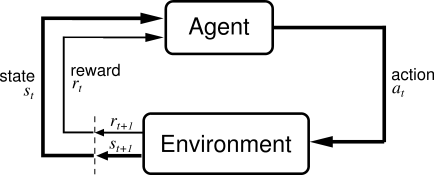
\includegraphics[width=0.6\textwidth]{reinforcement_learning}
\caption{Tranzi\c tia st\u arilor \^ in RL}
\end{figure}

\paragraph{}
Pentru a ac\c tiona optim, agentul trebuie s\u a ia \^ in considerare dependen\c ta pe termen lung a ac\c tiunilor sale (s\u a maximizeze recompensa viitoare), chiar dac\u a r\u asplata imediat\u a este asociat\u a cu o valoare negativ\u a. Astfel, RL este potrivit pentru probleme unde exist\u a un compromis care include o recompens\u a \^ intre o dependen\c t\u a pe termen lung \c si una pe termen scurt. A fost aplicat cu succes \^ in diverse situa\c tii precum controlul automat de robo\c ti, telecomunica\c tii, jocuri ATARI \c si recent jocul Go \cite{silver2016mastering}.

\paragraph{}
Jiwei Li et al. propun \^ in articolul lor, Deep Reinforcement Learning for Dialogue Generation \cite{DBLP:journals/corr/LiMRGGJ16}, utilizarea metodelor de RL pentru \^ inv\u a\c tare de limbaj. Plec\^ and de la aceea\c si arhitectur\u a HRED, descris\u a \^ in capitolul 3, se poate ca prin folosirea unor reguli euristice de determinare a recompensei, pe baza r\u aspunsurilor oferite de c\u atre chatbot, re\c teaua s\u a fie capabil\u a s\u a ofere r\u aspunsuri mai clare, contextuale \c si corect gramaticale. Astfel, articolul propune trei metode de recompens\u a pentru cuantificarea calit\u a\c tii unui r\u aspuns:

\begin{itemize}
	\item \(r_1\), care recompenseaz\u a modelul pentru r\u aspunsuri care nu fac parte dintr-un subset de r\u aspunsuri manual alese ca fiind monotone (I'm sorry, I don't know, Yes, No, etc.)
	\item \(r_2\), care recompenseaz\u a sistemul pentru nerepetarea aceluia\c si r\u aspuns consecutiv de mai multe ori la r\^ and
	\item \(r_3\), care recompenseaz\u a corectitudinea gramatical\u a \c si coeren\c ta r\u aspunsului
\end{itemize}


R\u asplata final\u a va fi o medie ponderat\u a \^ intre cele trei recompense:
\begin{center}
\(\lambda_1 r_1 + \lambda_2 r_2 + \lambda_3 r_3\)
\end{center}

unde \(\lambda_1 + \lambda_2 + \lambda_3 = 1\), iar \(\lambda_1 = 0.25, \lambda_2 = 0.25, \lambda_3 = 0.5\)

\paragraph{}
Folosind RL, autorii respectivi demonstreaz\u a c\u a rezultatele pot fi considerabil \^ imbun\u at\u a\c tite. De aceea, extinderea modelului curent pentru a folosi RL reprezint\u a una dintre principalele posibilele dezvolt\u ari dorite.

\section{Mecanisme de aten\c tie}

\paragraph{}
Mecanismele de aten\c tie \cite{DBLP:journals/corr/BahdanauCB14} pentru o RNA sunt puternic bazate pe cele vizuale existente la om. Aten\c tia vizual\u a uman\u a, de\c si este bine studiat\u a \c si exist\u a diverse modele, toate se rezum\u a la a fi capabile s\u a se concentreze asupra unei anumite regiuni dintr-o imagine cu o rezolu\c tie sporit\u a, pe c\^ and imaginea de fundal este perceput\u a cu o rezolu\c tie mai scazut\u a, punctul focal fiind ajustat de-a lungul timpului. 

\paragraph{}
Pentru a observa utilitatea acestora, se pleac\u a de la arhitectura standard seq2seq ca exemplu. Precum a fost descris \^ in Capitolul 3, codorul are rolul de a captura \^ in\c telesul \^ intregii fraze de intrare \^ intr-un vector de lungime fix\u a, care mai apoi va fi folosit pentru inferen\c t\u a. Pare nerezonabil ca \^ intreaga informa\c tie s\u a fie stocat\u a \^ intr-un singur vector, \^ in special dac\u a lungimea frazei este mare. LSTM se presupune c\u a rezolv\u a cu succes problema dependen\c tei temporale a unei secven\c te, \^ ins\u a \^ in practic\u a aceste neajunsuri \^ inc\u a apar atunci c\^ and lungimea acesteia este prea mare. O rezolvare plauzibil\u a poate fi oferit\u a prin folosirea RNAR bidirec\c tionale, care produc rezultate semnificativ mai bune. 

\paragraph{}
Aici intervin mecanismele de aten\c tie. Acestea nu mai captureaz\u a \^ intreaga informa\c tie a codorului \^ intr-un singur vector fix ci permit decodorului s\u a observe diferite p\u ar\c ti ale frazei surs\u a la fiecare pas al gener\u arii. Ceea ce este important este c\u a modelul \^ inva\c t\u a singur ce informa\c tie trebuie selectat\u a pe baza a ceea ce a fost produs p\^ an\u a \^ in acel moment \c si al intr\u arii (Figura 5.2).

\begin{figure}[H]
\centering
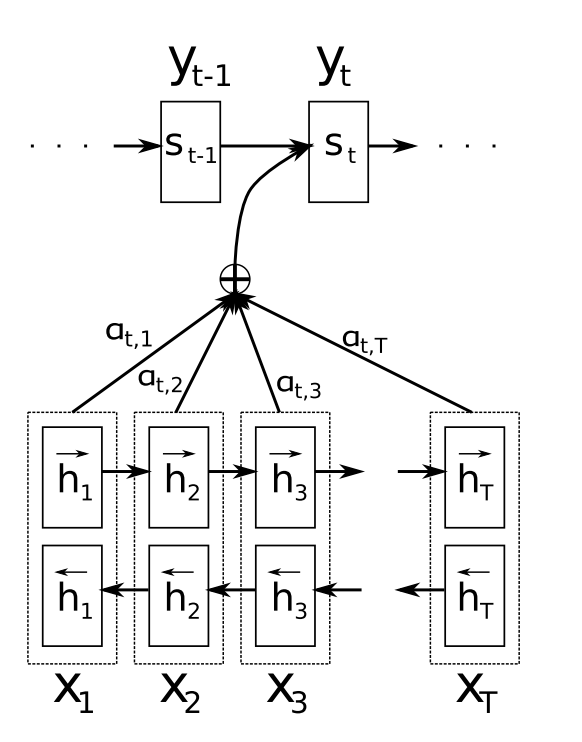
\includegraphics[width=0.4\textwidth]{attention_model}
\caption{Mecanism de aten\c tie}
\end{figure}

\paragraph{}
\^ In figura de mai sus, \(y\) reprezint\u a ie\c sirea generat\u a de c\u atre decodor iar \(x\) cuvintele corespunz\u atoare frazei de intrare. Aspectul cel mai important este c\u a fiecare ie\c sire \(y_t\) depinde acum de o combina\c tie ponderat\u a (valorile \(a\)) a tuturor st\u arilor din codor, \c si nu doar de ultima. De exemplu, dac\u a \(a_{3,2}\) este un num\u ar mare, asta \^ inseamn\u a c\u a decodorul este foarte atent la cea de-a doua stare de intrare atunci c\^ and este produs al treilea cuv\^ ant. Ponderile \(a\) sunt deobicei normalizate astfel \^ inc\^ at suma lor s\u a fie egal\u a cu \(1\)\footnote{Distribu\c tie a st\u arilor de intrare}. 

\paragraph{}
Costul ata\c sat acestor mecanisme este destul de mare. Pentru fiecare combina\c tie intrare-ie\c sire trebuie calculat\u a o valoare de aten\c tie \c si stocat\u a. Acest lucru este contraintuitiv, deoarece aten\c tia uman\u a se presupune c\u a economise\c ste resurse computa\c tionale focaliz\^ and doar ce este important. Modelul prezentat analizeaz\u a totul \^ in detaliu \^ inainte de a decide ce este important. Totu\c si, acest lucru nu a \^ impiedicat ca mecanismele de aten\c tie s\u a devin\u a at\^ at de populare \c si s\u a produc\u a rezultate bune pentru o multitudine de sarcini.

\section{Setul de date}

\paragraph{}
Unul dintre aspectele esen\c tiale de care puterea de procesare Deep Learning profit\u a este cantitatea mare de date. Dac\u a modelele tradi\c tionale de Machine Learning nu reu\c seau s\u a exploateze cre\c sterea volumului de date, modelele Deep Learning nu sufer\u a de aceast neajuns (Figura 5.3). Acest fapt este explicabil prin simplul fapt c\u a modelele tradi\c tionale nu erau suficient de complexe pentru a captura distribu\c tia datelor de intrare. Datorit\u a complexit\u a\c tii sporite a modelelor deep learning, care au avut parte de o explozie de popularitate odat\u a cu cre\c sterea capacit\u a\c tii computa\c tionale, a memoriei pentru stocarea datelor \c si folosirea procesorului grafic pentru a paraleliza calculele pe mii de nuclee, acestea pot surprinde cu u\c surin\c t\u a distribu\c tia unui set de date cu multe \c sabloane. Av\^ and acest beneficiu la dispozi\c tie, modelul actual poate fi \^ imbun\u at\u a\c tit dac\u a este antrenat lu\^ and \^ in considerare o cantitate mai mare de triplete de fraze.

\begin{figure}[H]
\centering
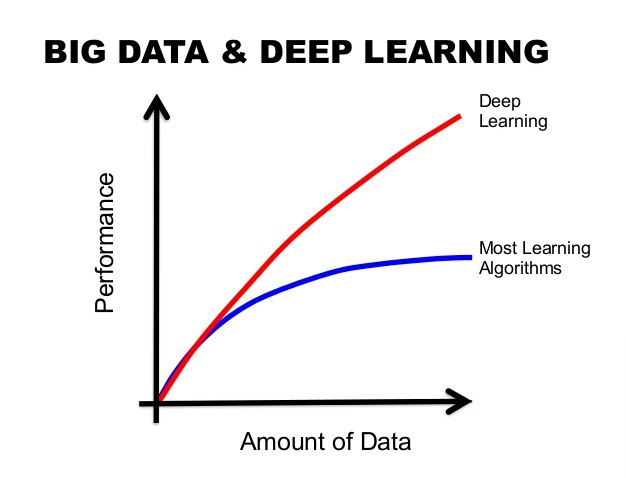
\includegraphics[width=0.6\textwidth]{data_scalability}
\caption{Scalabilitatea folosind Machine Learning vs Deep Learning}
\end{figure}

\paragraph{}
Desigur, o cantitate mai mare de date nu \^ inseamn\u a \^ intotdeauna c\u a rezultatul final este mai bun. \^ In urma experimentelor realizate, se poate observa o tendin\c t\u a a chatbot-ului de a fi \^ inclinat c\u atre r\u aspunsuri care se reg\u asesc \^ in setul de antrenare de un numar mare de ori, precum ``I'm sorry", ``I don't know" etc. Acest fenomen este explicat de faptul c\u a statistic vorbind aceste r\u aspunsuri se apropie foarte mult de media distribu\c tiei datelor de intrare. Acest lucru ridic\u a problema diversit\u a\c tii c\^ at \c si a calit\u a\c tii datelor care sunt furnizate sistemului. O solu\c tie plauzibil\u a este antrenarea folosind diverse seturi de date cunoscute ca fiind de referin\c t\u a pentru sarcini de procesare de limbaj natural, precum The Ubuntu Dialogue Corpus \cite{DBLP:journals/corr/LowePSP15}, \c si compararea cu modelul curent.




